\section{Search Results Page}

The majority of the complexity and development arguably lies within
the indexing processes of the search applicatio, but it is with the
\emph{actual Search Engine Results Page} (SERP) that the website users interact.

\begin{figure}
  \begin{center}
    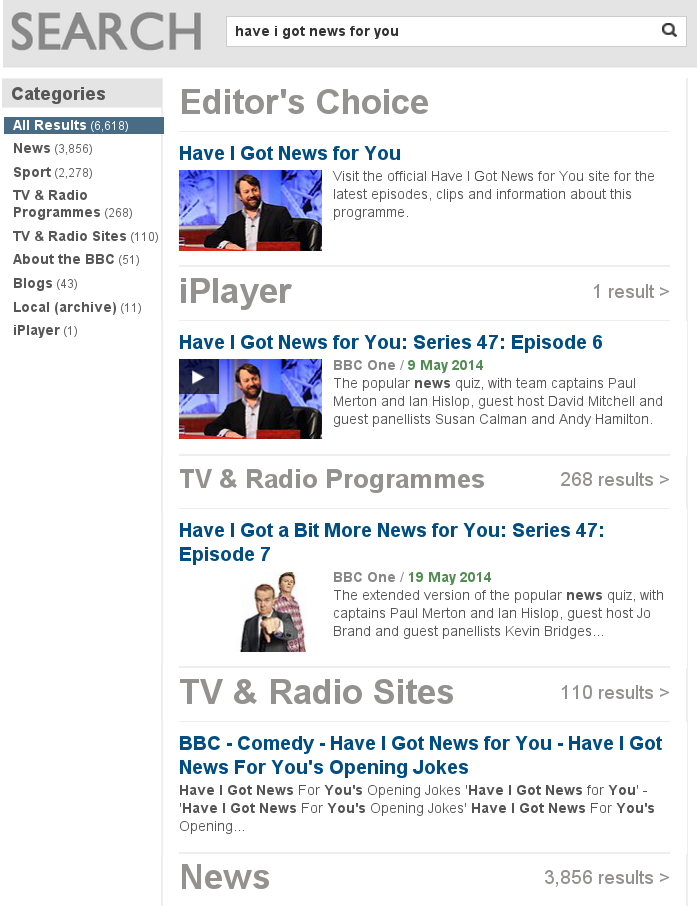
\includegraphics[width=\linewidth]{results-page.png}
  \end{center}
  \caption{Results page for BBC Search}
  \label{fig:search-page}
\end{figure}

The different categories/zones are shown on the left menu, with the
number of results found within each category also shown. The first results
are ``Editor's Choice'' results where the application
has matched manually-curated pages against the query. This module appears
as its own distinct category at the top of the list, but functionally
is a distinct feature to the ``organic'' results that follow below.

The organic results are broken into categories such that this ``All Results''
page reached after a search acts as a way to skim over each relevant
category.

The mix of ``iPlayer'' (episodes available to watch on iPlayer),
``TV \& Radio Programmes'' (microsites about programmes, series
and episodes past, present and forthcoming) and ``TV \& Radio Sites''
(web-crawled pages from legacy programme information sites) produces
a bit of redundancy that may confuse users and pushes non-programmes
results below the fold of the page on even desktop screens.

However, fuller analysis of the design and layout of the results page
is a subject for a separate and distinct study. Such an analysis
should certainly be part of the road map for any changes to the
results pages so as to give a broader view of how users interact
with the page and thus what behaviours of the search application
are desirable throughout the entire stack. In this study, the
primary concern is around the appearance and use of metadata
and linkable information.

There is no semantic markup in the results pages, but it might be
questionable as to whether any is needed as the search application
is not \emph{publishing} the data. However, the results page does
make \emph{use} of metadata about content to decorate and alter
the display of each result.

Every search result has the basic trio of title, summary and outgoing
link. Some results (where possible) are accompanied by a thumbnail
image to give more indications about the content they represent. Certain
types of results have a date attached, giving some idea of how recent
the item is. Dates are useful to help users assess the relevance
of results -- a user can dismiss older content if they know they
are looking for new information only.

Some results also carry categorisation specific to their respective
domains. News results are marked with which area of the news
website owns the article (e.g. Politics, Technology, Education). Similarly,
programmes are annotated with which TV or Radio service owns
that programme -- a concept known as the \emph{master brand} of a programme,
e.g. the programme \emph{Doctor Who} is known as a \emph{BBC One} programme.

Video and audio results have call-to-action icons added to indicate
the item can be watched or listened to respectively. These kinds
of annotations are important to give users ideas of how they would
be interacting with the item. This, again, can help a user assess more
accurately if the result is the one for which they are looking.

Currently, whether the item is textual, video or audio is driven by
a metadata field known as \emph{media type}. This classifies the content
into a set of predetermined types and the application uses rules
along the lines of ``if the media type is \emph{video} then add a play icon''.

This works well enough for programmes, but there are areas where
a class-based distinction might not be so clear cut. For example, some articles
on BBC News are accompanied by a video. Is this item textual or a video?
The current search application does not apply a play icon because the
article is classified as textual, as all news story pages are.
